\subsection{Redes Neuronales Recurrentes más comunes}

Existen diversas formas como construir \textit{Redes Neuronales Recurrentes}, estas pueden producir una
salida en cada paso de tiempo o tener solo una al final de la recurrencia  o tener
conexiones entre unidades ocultas. La manera más común de implementar una \textit{RNN} está ilustrada en la
figura \ref{fig:rnn_cfga}. En esta figura, cada etapa de la recurrencia es retroalimentada por la
activación del estado oculto previo. Así, $h^{(t)}$ contiene información codificada de elementos
previos de la secuencia que puede ser usada en el futuro para obtener una salida $O^{(t+1)}$. En la
figura \ref{fig:rnn_cfgb} se
cambia la retroalimentación de $h^{(t)}$ por $o^{(t)}$. Nótese que en este caso, la red es entrenada
para obtener un valor en específico $o^{(t)}$ lo que provocaría que gran parte de la información de
los estados ocultos pasados $h^{(t-1)}, h^{(t-2)}, ...$ no se transmita.
La diferencia entre los dos esquemas anteriores es que
la red \ref{fig:rnn_cfga} es entrenada para decidir que información debe transmitir en el futuro a través
de los estados ocultos, en cambio, en la figura \ref{fig:rnn_cfgb} cada estado esta conectado con el
pasado a través de la predicción del paso anterior, perdiendo así gran parte de la información
codificada en cada estado oculto $h^{(t)}$. Este no sería un problema si la salida $O^{(t-1)}$ fuese
lo suficientemente enriquecedora y en altas dimensiones.

% \begin{figure}[!ht]
% \centering
% 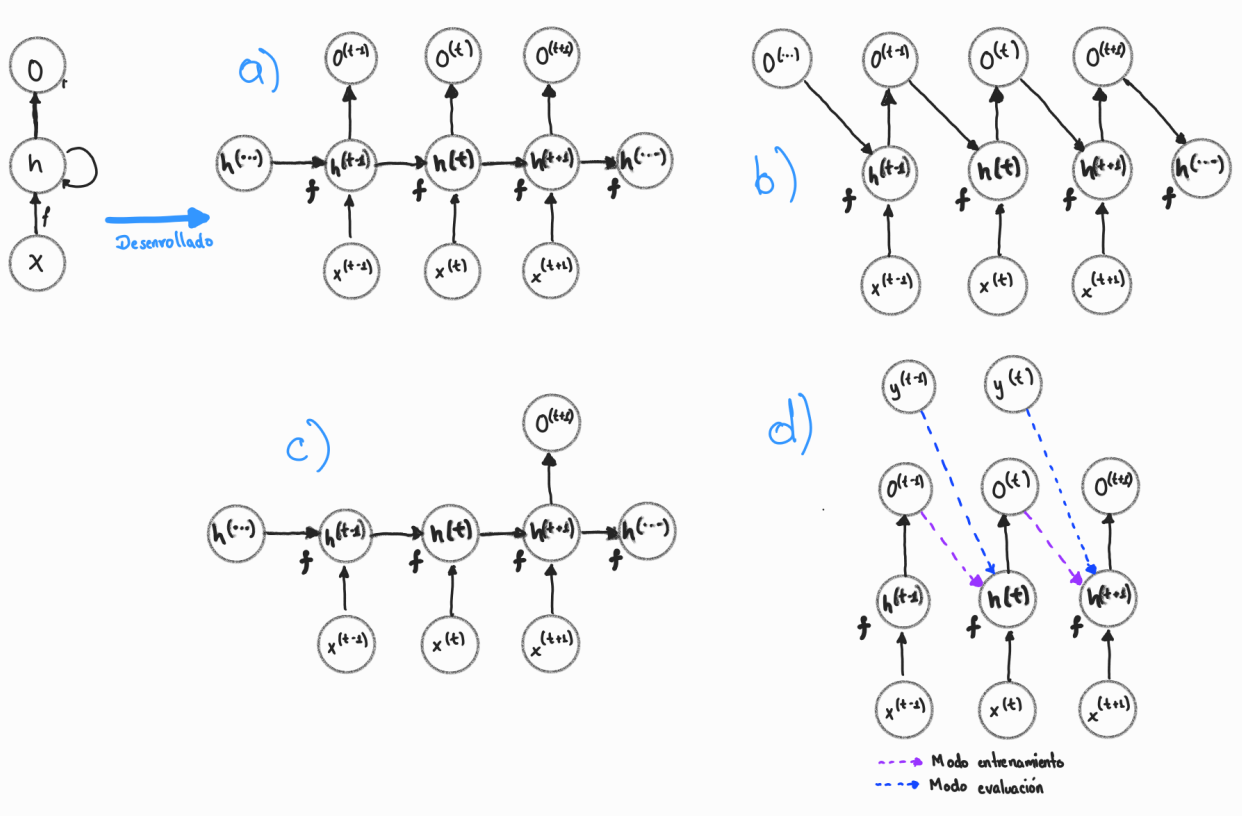
\includegraphics[width=.8\textwidth]{Chapters/2. Transformer/Figures/rnn/rnn_cfg.png}
% \caption[RNN - CFG]{Distintos tipos de RNNs. \textbf{a)} Las activaciones de las capas ocultas $h^{(t)}$
% alimentan al nodo siguiente, cada etapa de la recurrencia genera una salida $o^{(t)}$ \textbf{b)}
% Cada nodo es alimentado por las salidas de cada estado oculto $o^{(t)}$. \textbf{c)} Al final de la
% recurrencia solo tiene una salida $o^{(T)}$, puede ser usada para resumir/predecir un valor de una
% secuencia. \textbf{d)} Teacher Forcing. En modo de entrenamiento cada nodo en el tiempo $t$ es
% retroalimentado por la salida correcta $y^{(t-1)}$, en modo evaluación es retroalimentado por las
% salidas del modelo $O^{(t-1)}$}
% \label{fig:rnn_cfg}
% \end{figure}

\begin{figure}[!ht]
    \centering
    \begin{subfigure}[b]{0.49\textwidth}
        \centering
        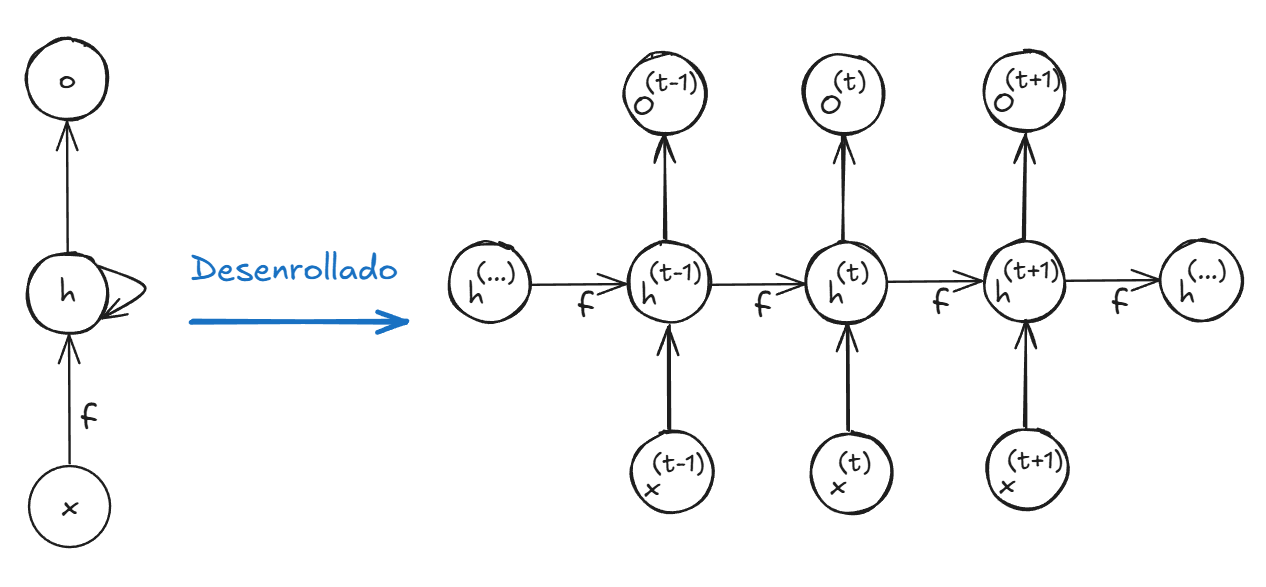
\includegraphics[width=\textwidth]{Chapters/2. Transformer/Figures/rnn/rnn_cfga.png}
        \caption{Las activaciones de las capas ocultas $h^{(t)}$
        alimentan al nodo siguiente, cada etapa de la recurrencia genera una salida $o^{(t)}$.}
        \label{fig:rnn_cfga}
    \end{subfigure}
    \hfill
    \begin{subfigure}[b]{0.4\textwidth}
        \centering
        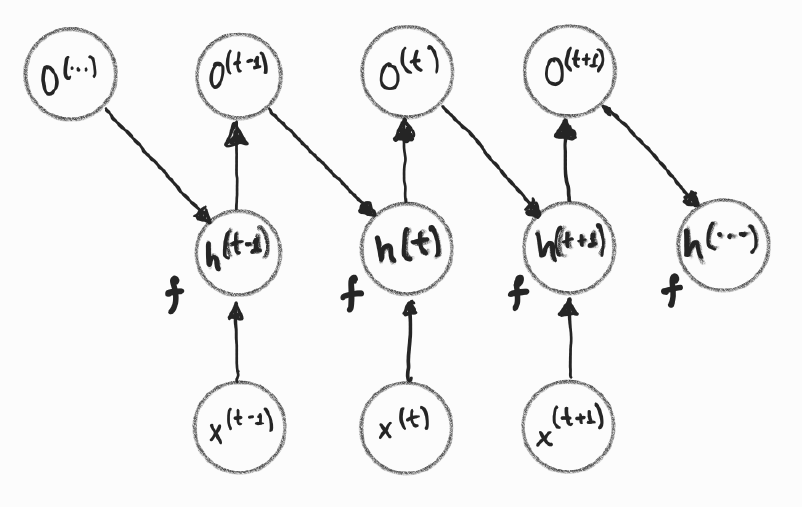
\includegraphics[width=\textwidth]{Chapters/2. Transformer/Figures/rnn/rnn_cfgb.png}
        \caption{Cada nodo es alimentado por las salidas de cada estado oculto $o^{(t)}$.}
        \label{fig:rnn_cfgb}
    \end{subfigure}

    \begin{subfigure}[b]{0.4\textwidth}
        \centering
        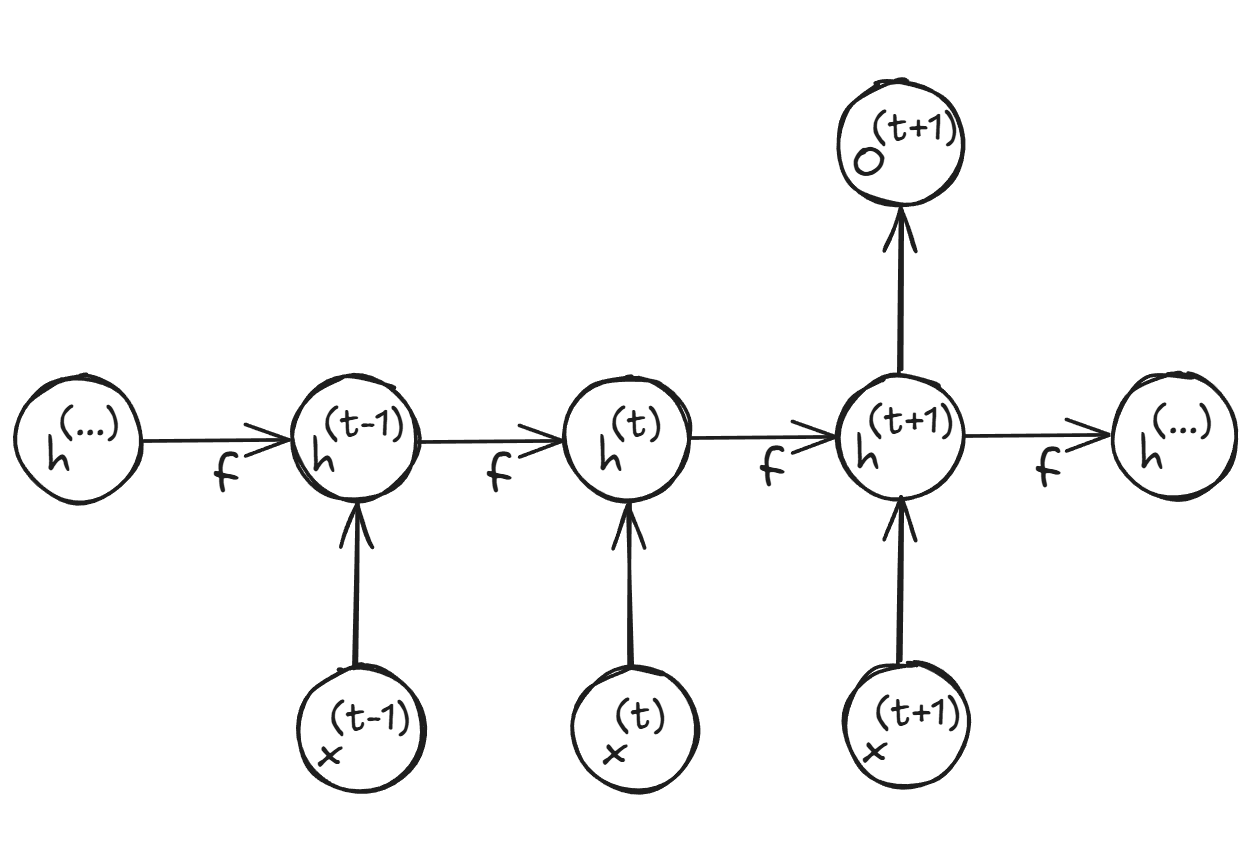
\includegraphics[height=0.63\textwidth]{Chapters/2. Transformer/Figures/rnn/rnn_cfgc.png}
        \caption{Al final de la recurrencia solo tiene una salida $o^{(T)}$, puede ser usada para
        resumir/predecir un valor de una secuencia.}
        \label{fig:rnn_cfgc}
    \end{subfigure}
    \hfill
    \begin{subfigure}[b]{0.49\textwidth}
        \centering
        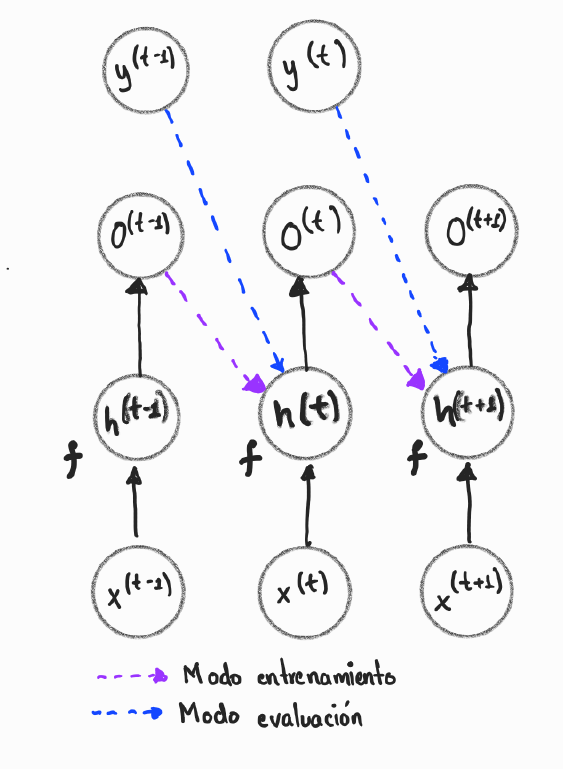
\includegraphics[height=0.6\textwidth]{Chapters/2. Transformer/Figures/rnn/rnn_cfgd.png}
        \caption{Teacher Forcing. En modo de entrenamiento cada nodo en el tiempo $t$ es
        retroalimentado por la salida correcta $y^{(t-1)}$, en modo evaluación es retroalimentado por las
        salidas del modelo $O^{(t-1)}$.}
        \label{fig:rnn_cfgd}
    \end{subfigure}

    \caption{Distintos tipos de RNNs.}
    \label{fig:three graphs}
\end{figure}


Por otro lado, la \textit{RNN} representada en la figura \ref{fig:rnn_cfgc} tiene una sola salida al
final de la recurrencia.
Al contrario de las anteriores, este tipo de redes pueden ser usadas para resumir
información contenida en la secuencia para finalmente predecir un único valor final.
El \textit{Análisis de Sentimiento} en textos es una tarea común que puede ser representada con este esquema
de red. En la figura \ref{fig:rnn_cfgd} vemos un modelo de \textit{RNN} entrenado mediante el proceso de
Teacher Forcing; durante el entrenamiento la red es retroalimentada con las salidas
esperadas del modelo $y^{(t)}$ en el tiempo $t+1$. La ventaja de esta red es que al ser eliminadas
las conexiones entre estados ocultos, las funciones de pérdida basadas en comparar la predicción en
el tiempo $t$ con el valor objetivo $y^{(t)}$ pueden ser desacopladas. Por tanto, el entrenamiento
puede ser paralelizado al calcular el gradiente para cada tiempo $t$ por separado, puesto que ya
tenemos el valor ideal para esta salida.

Finalmente, en la figura \ref{fig:rnn_cfge} la \textit{Red Neuronal Recurrente} es modificada para esta vez
no procesar una secuencia, sino, procesar un solo vector en cada paso. El estado oculto
previo $h^{(t-1)}$ retroalimenta al siguiente paso $t$ así como la predicción esperada $y^{(t)}$, que
a su vez, es usada para calcular la función de costo del paso anterior $L^{(t-1)}$. Esta estructura de
red puede ser implementada en tareas como \textit{Image Captioning}, en donde la entrada es una imagen y la salida
una secuencia de palabras que describen esta misma.

\begin{figure}[!ht]
\centering
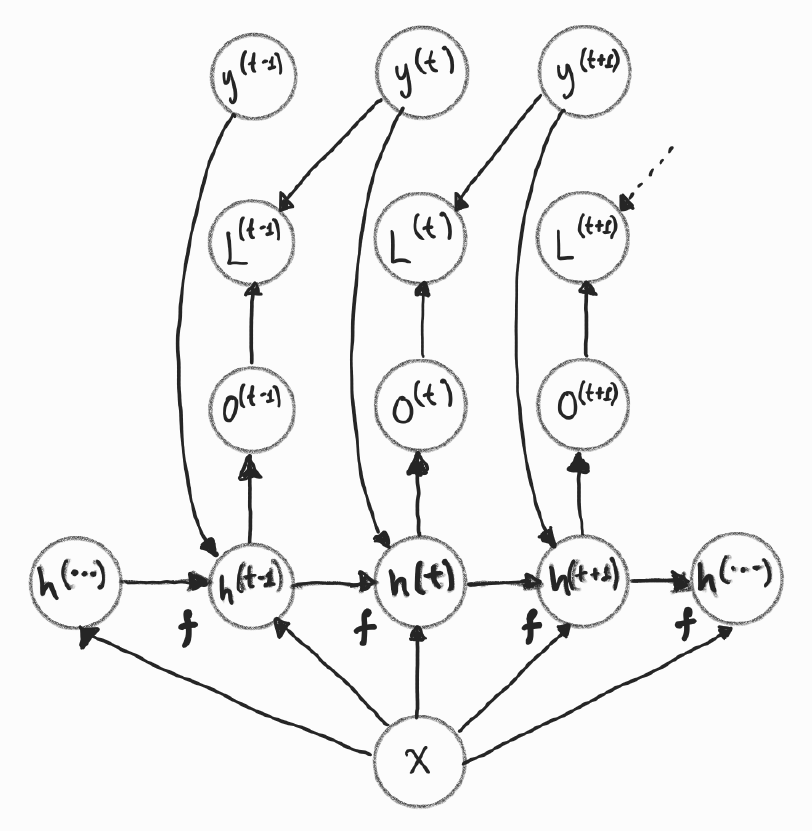
\includegraphics[width=.4\textwidth]{Chapters/2. Transformer/Figures/rnn/rnn_cfge.png}
\caption{Modelo usado para tareas de \textit{Image Captioning}, la entrada es una
sola imagen y la red predice una secuencia de palabras que describen dicha imagen La salida esperada
$y^{(t)}$ sirve como objetivo para la función de costo del paso anterior y como entrada en cada paso.}
\label{fig:rnn_cfge}
\end{figure}


Los modelos ejemplificados anteriormente son construidos de forma \textit{causal}, es
decir, la secuencia es procesada en un solo sentido en donde la información pasada es transmitida
hacia estados futuros. Sin embargo, este flujo de información puede ser insuficiente para resolver
todas las tareas. En \textit{Modelo de Lenguaje} se aprende la estructura estadística del lenguaje con el
que fue entrenado y su meta es predecir la siguiente palabra, n-grama o letra dado un contexto antes
visto. En otros términos, dada una secuencia de texto de longitud
$T$ $x^{(1)}, x^{(2)}, ..., x^{(T)}$
con $x \in \mathcal{R}^{1 \times d}$ donde $d$ es la dimensión de la codificación de las palabras,
la meta es predecir la probabilidad conjunta de la secuencia:

\begin{equation}
    P(x^{(1)}, x^{(2)}, ..., x^{(T)}) = \prod_{t=1}^{T} P(x^{(t)} | x^{(t)}, \dots , x^{(t-1)})
\end{equation}

Con ello, un modelo de lenguaje basado en \textit{Redes Neuronales Recurrentes} es capaz de predecir
un siguiente elemento $\hat x^{(t)}$ simplemente obteniéndolo de la secuencia mediante:

\begin{equation}
    \hat x^{(t)} \approx P(x^{(t)} | x^{(t-1)}, \dots, x^{(1)}) \approx P(x^{(t)} | h^{(t-1)})
\end{equation}

\noindent donde $h^{(t-1)}$ es el estado oculto que almacena la información pasada hasta el tiempo $t$
tal y como se definió en \ref{eq:rnnh}.

Sin embargo, la información previa de la secuencia codificada en $h^{(t)}$ no siempre contiene los
elementos necesarios para que el modelo pueda predecir correctamente el siguiente elemento,
observe la siguiente oración:

\begin{center}
    % \tiny
    << \textit{Ella estaba muy \_\_\_\_\_, después de que Rosario vió el amanecer en la playa } >>
\end{center}

\noindent en la oración anterior, el espacio en blanco puede ser completado con algún adjetivo calificativo;
\textit{contenta}, \textit{enojada}, \textit{maravillada}, etc. Gracias a la información provista por
la parte final de la oración, podemos deducir que de las 3 opciones la menos probable de
elegir es \textit{enojada}. Es decir, usamos información del futuro que no pudo haber sido vista por
una red (que procesa la información en forma causal) para tomar la mejor elección. Una ligera
modificación fácilmente aplicable a estos modelos es que las secuencias sean procesadas
en ambas direcciones, las \textbf{Redes Neuronales Recurrentes Bidireccionales}
\cite{Schuster}.

Una \textit{RNN Bidireccional} procesa la secuencia en ambos sentidos (una \textit{RNN} en un
sentido y otra en el otro), capturando información del
pasado en el estado oculto $\overrightarrow{h}^{(t)}$  cuando la recurrencia es del inicio al final
de la secuencia e información del futuro en $\overleftarrow{h}  ^{(t)}$ cuando la recurrencia es del
final al inicio de la secuencia. Finalmente, el estado oculto $h^{(t)}$ es una concatenación de ambos
estados $\overrightarrow{h}^{(t)}$ y $\overleftarrow{h}^{(t)}$, vea la ecuación \ref{eq:rrnbi}.
Por lo cual, la salida $o^{(t)}$ ahora puede ser calculada con información tanto del futuro como del pasado
\ref{eq:rrn_out}.

\begin{equation}
\begin{split}
    \overrightarrow{h}^{(t)} = f(x^{(t)}, \overrightarrow{h}^{(t-1)}; \theta_f)\\
    \overleftarrow{h}^{(t)} = f(x^{(t)}, \overleftarrow{h}^{(t+1)}; \theta_b)\\
    h^{(t)} = Concat(\overrightarrow{h}^{(t)}, \overleftarrow{h}^{(t)})
\end{split}
\label{eq:rrnbi}
\end{equation}

\begin{equation}
        o^{(t)} = g(h^{(t)}; \theta_{out})
\label{eq:rrn_out}
\end{equation}
